\documentclass[a4paper,12pt]{article}
\usepackage[catalan]{varioref}
\usepackage{setspace}
\usepackage[margin=2.54cm]{geometry}
\usepackage{pdfpages}
\usepackage[utf8]{inputenc}
\usepackage[catalan]{babel}
\usepackage{graphicx,subcaption}
\usepackage{graphics}
\usepackage{lscape}
\usepackage{pdflscape}
\usepackage{float}
\usepackage{textcomp}
\usepackage{amsmath}
\usepackage{hyperref}
\usepackage{subcaption}
\usepackage{pgfplots}
\usepackage{tikz}
\usepackage{fancyvrb}
\usepackage{parskip}
\usepackage{changepage}
\usepackage{enumitem}
\usepackage{tcolorbox}
\usepackage[all]{hypcap}
\usepackage{xcolor}
\usepackage{listings}
\definecolor{green}{HTML}{228B22}
\definecolor{orange}{HTML}{FFC107}
\usepackage{color}
\definecolor{dkgreen}{rgb}{0,0.6,0}
\definecolor{gray}{rgb}{0.5,0.5,0.5}
\definecolor{mauve}{rgb}{0.58,0,0.82}
\lstset{escapeinside={<@}{@>}}

\hypersetup{
    colorlinks,
    citecolor=black,
    filecolor=black,
    linkcolor=black,
    urlcolor=blue
}


\lstset{frame=tb,
    language=python,
    aboveskip=3mm,
    belowskip=3mm,
    showstringspaces=false,
    columns=flexible,
    basicstyle={\small\ttfamily},
    numbers=none,
    numberstyle=\tiny\color{gray},
    keywordstyle=\color{blue},
    commentstyle=\color{dkgreen},
    stringstyle=\color{mauve},
    breaklines=true,
    breakatwhitespace=true, tabsize=3
}
\title{
	\begin{center}
	\vspace{3cm}
	\includegraphics[width=11cm, height=3cm]{images/Logo-nou-eps.jpg}
	\end{center}
	\begin{center}
	\line(1,0){340}
	\end{center}		
	TREBALL DE FI DE GRAU\\
	\vspace{2mm}
	\Large L'alzheimer contra la IA. Qui guanyarà?\\
	\line(1,0){340}
	\vspace{2.5cm}
	}

\author{Marc Cervera Rosell - 47980320C \vspace{1cm}}


\date{Curs acadèmic 2022-23\vspace{0.5cm} \\Grau en Enginyeria Informàtica}
\onehalfspacing

\begin{document}
\thispagestyle{empty}
	\begin{titlepage}
		\maketitle
		\thispagestyle{empty}
	\end{titlepage}
	\cleardoublepage
	\newpage
\thispagestyle{empty}
\tableofcontents
\thispagestyle{empty}
\listoffigures
\thispagestyle{empty}

\newpage
\setcounter{page}{1}
\pagestyle{plain}
\section*{Introducció}
\addcontentsline{toc}{section}{Introducció}
Detectar de manera precoç l'Alzheimer en una persona és un dels desafiaments que enfronta la medicina del segle XXI. Els mètodes utilitzats avui dia per a la detecció precoç d'aquesta malaltia són molt costosos i requereixen una copiosa inversió de temps i recursos. Tot i que la detecció d'aquesta malaltia és un desafiament realment complicat, és crucial per poder garantir un tractament i una qualitat de vida adequats per als pacients que, per desgràcia, pateixen els efectes d'aquesta malaltia.\\
Durant la realització d'aquest treball de final de grau, s'investigarà de quina manera pot ajudar la intel·ligència artificial en la detecció primerenca de la malaltia d'Alzheimer a partir d'imatges de ressonància magnètica cerebral (MRI en anglès). L'aplicació del \textit{Machine Learning} en el camp de la salut, i més concretament en el cas que tracta aquest treball (l'Alzheimer), és una tècnica que augura moltes esperances de facilitar la detecció precoç d'aquesta terrible malaltia. Les esperances es basen en el fet que l'ús de la intel·ligència artificial pot ajudar, com s'ha esmentat, a detectar de manera primerenca aquesta patologia d'una manera no invasiva ni dolorosa per al pacient, cosa que podria millorar molt significativament la qualitat de vida i reduir els costos que suposa el diagnòstic tardà i el tractament.\\
Com s'explicarà més endavant en aquest document, les xarxes neuronals convolucionals, s'han convertit en la tècnica que proporciona més esperances a les comunitats científica i sanitària, perquè són capaces d'extreure les característiques complexes d'una ressonància magnètica i utilitzar-les per ajudar al professional mèdic corresponent a confirmar o descartar el diagnòstic d'Alzheimer.\\
Per dur a terme l'objectiu principal d'aquest treball de final de grau, es farà ús de la tècnica d'aprenentatge supervisat, per entrenar una sèrie de dades etiquetades que “ensenyaran” a la xarxa convolucional a diferenciar entre quatre nivells possibles de demència per Alzheimer. Aquests quatre nivells són; no dement, dement molt lleu, dement lleu, dement moderat.\\
L'estructura que seguirà el treball consta de vuit blocs, el primer dels quals contindrà informació sobre la malaltia d'Alzheimer. El segon, conformarà el bloc del marc teòric computacional, en el qual constarà informació detallada sobre la tecnologia emprada en la realització del treball. El tercer bloc tractarà sobre les aplicacions de la intel·ligència artificial en el camp de la salut. Concretament, es comentaran diversos aspectes relacionats amb l'aplicació de la tecnologia per al diagnòstic i tractament de la malaltia. El següent bloc contindrà informació sobre el desenvolupament de la proposta, tot mostrant anàlisis gràfiques de les mètriques de rendiment de la xarxa neuronal com una anàlisi exhaustiva d'en quines parts de les imatges es fixa el model en el moment de fer la classificació de la imatge d'input. Seguidament, el cinquè bloc contindrà les conclusions extretes després de realitzar la investigació. El sisè bloc contindrà els annexos del treball on es definiran alguns conceptes que no hagin pogut quedar clars en el moment de la redacció d'aquest document. En el penúltim bloc, constaran els agraïments a les persones que han fet possible la realització i la finalització exitosa d'aquest treball. Finalment, el vuitè i últim bloc, especificarà les referències bibliogràfiques que han estat necessàries per a la recerca.
\section*{\textit{Abstract}}
\addcontentsline{toc}{section}{Abstract}
\textit{This document will explain the development process of an artificial intelligence model able to identify up to four levels of dementia caused by Alzheimer's disease. These levels are; “non-demented”, “ver mild demented”, “mild demented” and “moderate demented”.\\
The main aim of this thesis is to give to the health workers a new tool to get helped to confirm or discart the Alzheimer's diagnosis, but the most important is not to give a diagnosis tool. The most essential, is to give a new tool that allows early diagnosis to give to the patients the best life quality and reduce the costs of late diagnosis.}
\section*{Marc teòric clínic}
\addcontentsline{toc}{section}{Marc teòric clínic}
\subsection*{Quan i qui va descobrir l'Alzheimer?}
\addcontentsline{toc}{subsection}{Quan i qui va descobrir l'Alzheimer?}
Abans d'entrar de ple en què és l'Alzheimer, quins símptomes presenta, etc. cal fer una mica la vista enrere a la història per saber qui i quan va descobrir aquesta malaltia.\\
A principis del segle XX, concretament l'any 1901, el psiquiatre alemany \textit{Alois Alzheimer}, es va topar amb uns estranys símptomes en una pacient anomenada \textit{Auguste Deter} de cinquanta-un anys. Aquesta dona patia pèrdua de memòria a curt termini i al·lucinacions auditives, cosa que va deixar perplex al doctor \textit{Alzheimer}. Descobrir els motius del comportament de la seva pacient, es va convertir en l'obsessió del doctor i, cinc anys després, quan la pacient \textit{Auguste Deter} va morir en un asil de la ciutat de \textit{Frankfurt}, \textit{Alzheimer} va conservar dues coses que van ser elements clau en la història d'aquesta malaltia. Els elements conservats pel doctor, varen ser l'historial clínic de la pacient i estudis del seu cervell. El Dr. \textit{Alzheimer} va portar a \textit{Munich}, concretament al laboratori d'\textit{Emil Kraepelin} un pioner en l'àrea psiquiàtrica, els seus descobriments amb la finalitat de poder començar una investigació encara més rigorosa.\\
Durant l'autòpsia del cervell de la seva pacient, el doctor \textit{Alzheimer} va descobrir que l'escorça cerebral era més estreta del normal i hi havia dos tipus d'anomalies notables: plaques d'amiloide, que són acumulacions de proteïnes entre les neurones, i cabdells d'una altra proteïna anomenada tau. Aquestes anomalies estan relacionades amb la disminució de la funció neuronal.\\
El doctor va presentar el cas de la seva pacient en una reunió de psiquiatria, però no va generar molt interès. No obstant això, l'any 1910, el Dr. \textit{Kraepelin} va començar a referir-se a aquella malaltia com la “malaltia d'Alzheimer”. El Dr. \textit{Alzheimer} no podia imaginar que aquell primer contacte amb aquella dona de cinquanta-un anys iniciaria una llarga i difícil batalla (batalla que avui dia encara continua amb investigadors a primera línia de batalla) per descobrir tots els símptomes i una cura per la causa de demència més comuna.\\
El Dr. \textit{Alois Alzheimer} va morir l'any 1915, però el seu llegat en el camp de la biomedicina encara és viu. El doctor és reconegut no solament per la seva descripció inicial d'una afecció, sinó també per ser un exemple d'investigador clínic. Va establir un estàndard per comprendre els desordres neurodegeneratius en mantenir una estreta relació amb els seus pacients i utilitzar eines científiques per explicar com els símptomes es relacionen amb els canvis físics del cervell.
\subsection*{Qué és l'Alzheimer i quins factors contribueixen a la seva aparició?}
\addcontentsline{toc}{subsection}{Qué és l'Alzheimer i quins factors contribueixen a la seva aparició?}
Atès que l'Alzheimer és la causa més comuna de demència, abans de definir res sobre la malaltia d'Alzheimer cal definir de manera clara que és la demència.\\
La demència, també coneguda com a trastorn neurocognitiu major, per definició, és un conjunt de símptomes que causen diverses infermetats. Aquests símptomes inclouen: afectacions en la memòria, afectacions en el comportament i afectacions en les habilitats socials de tal manera que dificulten les activitats quotidianes i la independència social.\\
Moltes de les infermetats que causen demència provoquen simptomatologia similar com pèrdua de la memòria i de l'orientació, comportament agressiu, problemes de parla i diverses afectacions a escala física. Cal remarcar que aquests símptomes es poden manifestar en moltes maneres, tot depenent de la persona afectada.\\
Un cop definit el terme de demència, es pot procedir a la definició d'Alzheimer.\\
L'Alzheimer és un tipus de demència que causa problemes amb la memòria, el pensament i el comportament. Els símptomes, generalment, es desenvolupen lentament i empitjoren amb el pas del temps, fins que són tan greus que interfereixen amb les tasques quotidianes. Cal remarcar que l'Alzheimer tot i ser la causa més comuna de demència no és l'única. En la següent imatge es pot observar un gràfic que de les demències més comunes:
\begin{figure}[H]
    \centering
    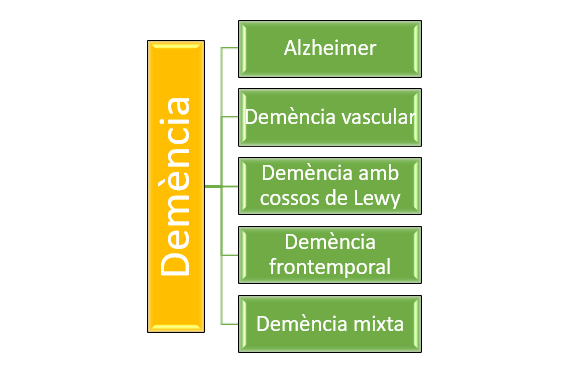
\includegraphics[scale = 0.5]{images/image_2023-03-08_172829369.png}
    \caption{Gràfic de les demències més comunes}
    \label{fig:demències}
\end{figure}
De tots els casos de demència que es diagnostiquen, s'atribueix un percentatge d'entre un 60\% i un 80\% a l'Alzheimer.\\
En cap cas aquesta malaltia és quelcom normal de l'envelliment, tot i que el factor de risc més important sigui el pas del temps, fet que implica fer-se gran. La majoria de les persones diagnosticades amb Alzheimer són majors de seixanta-cinc anys. Tot i que, cal assenyalar que la infermetat d'Alzheimer no afecta només a persones d'avançada edat, ja que al voltant de dues-centes mil persones, solament als Estats Units, menors de seixanta-cinc anys pateixen, de manera primerenca, aquesta malaltia.\\
L'Alzheimer és una infermetat progressiva. Això significa que empitjora amb el pas del temps. En les seves primeres etapes la pèrdua de memòria és lleu, però en l'etapa final, les persones perden la capacitat de mantenir una conversa i respondre a l'entorn.\\
Tenint en compte el factor de l'edat, existeixen una totalitat de quatre factors de risc.\\
El primer factor de risc, és l'herència. La malaltia pot ser hereditària on la meitat o més de cada generació està afectada per un gen dominant. En famílies on hi ha dues generacions consecutives amb membres afectats, els fills tenen un 50\% de probabilitats de patir Alzheimer, si viuen fins als vuitanta-cinc anys. En la forma esporàdica de l'infermetat el risc no es pot determinar, però augmenta si la persona té una constitució genètica amb el gen APO E-4. El risc solament augmenta en un 20\% sense la mutació del gen, un 47\% per aquells amb una mutació i un 91\% per aquelles persones amb dues mutacions del gen.\\
El segon factor de risc que pot contribuir a l'aparició d'Alzheimer, és un traumatisme cranial. Cal remarcar que els danys cerebrals en un pacient d'Alzheimer són majors, però el fet de patir un traumatisme cranial pot ser un factor desencadenant de la malaltia, tot i que la majoria de traumatismes cranials no són Alzheimer ni desencadenen la infermetat.
Un altre factor molt important a tenir en compte és el sexe. Com es veurà en la posteriorment a la secció d'estadístiques d'afectats per la infermetat, les dones són molt més propenses a tenir Alzheimer que els homes. De fet, s'estima només a Espanya, que en el 69\% dels casos d'Alzheimer el sexe afectat, és el sexe femení.\\
Com s'ha comentat anteriorment, els anys de vida és el factor més influent, però aquest deixa de ser un element dominant a partir dels noranta anys. A partir d'aquesta edat, el risc de patir Alzheimer disminueix, normalment. És capital posar en rellevància que, en cap cas, el nivell educatiu o intel·lectual, l'exposició continuada a l'alumini, els virus lents, les infeccions o viure en una zona rural o urbana són considerats factors de risc.
\subsection*{Quina simptomatologia ens ha de posar en alerta?}
\addcontentsline{toc}{subsection}{Quina simptomatologia ens ha de posar en alerta?}
Cent vint-i-dos anys després del descobriment de l'infermetat d'Alzheimer, per part del Dr. \textit{Alois Alzheimer}, la batalla per descobrir tots els símptomes de la malaltia continua. Avui en dia, encara no es coneix tota la simptomatologia que presenta la malaltia d'Alzheimer, però sí que hi ha determinats signes que han de posar en alerta a una persona i als seus familiars i amics.\\
Ara per ara, estan establerts deu símptomes que són senyals d'alarma per una possible demència per Alzheimer.\\
\textbf{La primera alarma és la pèrdua de memòria}. Especialment en els primers estadis de la infermetat, un dels principals senyals és oblidar informació recent, oblidar dates o esdeveniments importants, demanar la mateixa informació de manera reiterada, etc.\\
\textbf{El segon senyal d'alarma és la dificultat per planificar o resoldre problemes}. Algunes persones poden experimentar problemes per desenvolupar i seguir una rutina, treballar amb nombres seguir una recepta de cuina, concentrar-se en una tasca, etc.\\
\textbf{Com a tercera alarma, hi ha la dificultat per desenvolupar tasques habituals ja sigui a casa, a la feina o al temps d'oci}. Per exemple, es pot tenir dificultat per tasques tan habituals com rentar-se la cara, arribar d'un punt “A” a un punt “B”, sent el punt “B” una localització coneguda per la persona, administrar un pressupost o recordar les normes d'un joc.\\
\textbf{La quarta alerta és la desorientació en l'espaitemps}. Les persones amb Alzheimer obliden dates importants, les estacions de l'any i el pas del temps en general. També és molt probable que s'oblidin del lloc on es troben en aquell moment i de com han arribat allí.\\
\textbf{El cinquè senyal d'alarma és la dificultat de comprensió visual}. La comprensió visual es refereix a entendre imatges visuals i com els objectes es relacionen entre ells a l'entorn. Manca de comprensió visual també inclou la dificultat per llegir, jutjar distàncies, determinar el contrast de colors, etc.\\
\textbf{La sisena alarma és tenir impediments per utilitzar el llenguatge}. Tant en el llenguatge escrit com en la parla, les persones amb Alzheimer poden tenir dificultats per a seguir una conversa o que, per exemple, a mitja conversa parin sense tenir ni la més mínima idea del que estaven dient o que repeteixin reiteradament quelcom que acaben de dir fa escassos instants. També pot ser que no puguin trobar les paraules adients o que anomenin les coses per un nom incorrecte.\\
\textbf{L'alerta número set és col·locar objectes en llocs diferents de l'habitual i tenir dificultats per trobar-los}. Una persona afectada per la malaltia sol posar coses fora del seu lloc essent després completament incapaç de trobar-les. De vegades, és possible, que acusin altres persones de robar-los.\\
\textbf{L'antepenúltim senyal d'alarma és la disminució o la falta de judici}. La disminució de l'activitat cerebral pot provocar alteracions en la capacitat de jutjar el perill que comporta una acció i també pot provocar una alteració en la capacitat de prendre decisions.\\
\textbf{Com a penúltima alerta es troba la pèrdua d'iniciativa}. Cal subratllar, que aquest senyal és un “dels menys importants”, ja que la pèrdua d'iniciativa per participar en passatemps, activitats socials, projectes de treball o esports també es pot donar en altres malalties completament diferents de l'Alzheimer, com per exemple, la depressió.\\
\textbf{L'última alarma són els canvis d'humor o de personalitat}. Les persones amb la malaltia d'Alzheimer poden arribar a sospitar de tothom, ser persones agressives, temoroses o ansioses.
\subsection*{Quines fases té la malaltia?}
\addcontentsline{toc}{subsection}{Quines fases te la malaltia?}
En tot el món, professionals i cuidadors utilitzen l'escala de deteriorament global, desenvolupada pel Dr. Barry Reisberg, director del programa d'educació i investigació de la infermetat d'Alzheimer. Aquesta escala serveix per determinar en quin nivell de demència en què es troba la persona afectada d'Alzheimer.\\
Dividida en dos grans blocs; pre demència (estadis 1 a 3) i demència (estadis 4 a 7), l'escala consta de set estadis clínics diferents.\\
El punt d'inflexió on la persona ja no pot viure sense assistència continuada, és l'estadi 5.\\
A continuació, es presentaran els diferents blocs i estadis en un llistat i, posteriorment, s'explicaran les característiques de cada estadi.
\begin{itemize}
    \item Bloc pre demència
    \begin{itemize}
        \item Estadi 1: No demència observable.
        \item Estadi 2: Pèrdua de memòria relacionada amb l'edat.
        \item Estadi 3: Deteriorament cognitiu lleu.
    \end{itemize}
    \item Bloc de demència
    \begin{itemize}
        \item Estadi 4: Declivi cognitiu moderat. Demència lleu.
        \item Estadi 5: Declivi cognitiu moderadament sever. Demència moderada.
        \item Estadi 6: Declivi cognitiu sever. Demència moderadament severa
        \begin{itemize}
            \item Estadi 6A.
            \item Estadi 6B.
            \item Estadi 6C.
            \item Estadi 6D.
            \item Estadi 6E.
        \end{itemize}
        \item Estadi 7: Declivi cognitiu molt sever. Demència severa.
    \end{itemize}
\end{itemize}

\subsection*{Quin és el mètode diagnòstic actual?}
\addcontentsline{toc}{subsection}{Quin és el mètode diagnòstic actual?}

\subsection*{Quin és el tractament actual?}
\addcontentsline{toc}{subsection}{Quin és el tractament actual?}

\subsection*{De quines maneres es pot prevenir l'Alzheimer?}
\addcontentsline{toc}{subsection}{De quines maneres es pot prevenir l'Alzheimer?}

\subsection*{Estadístiques d'afectats en l'àmbit nacional i autonòmic}
\addcontentsline{toc}{subsection}{Estadístiques d'afectats a en l'àmbit nacional i autonòmic}

\subsection*{Principals associacions de lluita contra l'Alzheimer}
\addcontentsline{toc}{subsection}{Principals associacions de lluita contra l'Alzheimer}

\subsection*{Experiència personal amb la malaltia}
\addcontentsline{toc}{subsection}{Experiència personal amb la malaltia}

\section*{Marc teòric computacional}
\addcontentsline{toc}{section}{Marc teòric computacional}

\subsection*{Qué entenem per intel·ligència artificial?}
\addcontentsline{toc}{subsection}{Que entenem per intel·ligència artificial?}

\subsection*{Qué és el \textit{machine learning}?}
\addcontentsline{toc}{subsection}{Que és el \textit{machine learning}?}

\subsection*{Qué és una xarxa neuronal?}
\addcontentsline{toc}{subsection}{Qué és una xarxa neuronal?}

\subsubsection*{Qúe composa una xarxa neurona?}
\addcontentsline{toc}{subsubsection}{Qúe composa una xarxa neurona?}

\subsection*{Xarxes neuronals convolucionals (CNN)}
\addcontentsline{toc}{subsection}{Xarxes neuronals convolucionals (CNN)}

\subsection*{Entrenament de xarxes neuronals}
\addcontentsline{toc}{subsection}{Entrenament de xarxes neuronals}

\newpage

\section*{La intel·ligència artificial en la salut}
\addcontentsline{toc}{section}{La intel·ligència artificial en la salut}

\section*{Implementació de la proposta de treball i anàlisi de resultats}
\addcontentsline{toc}{section}{Implementació de la proposta de treball i anàlisi de resultats}

\subsection*{Disseny dels experiments}
\addcontentsline{toc}{subsection}{Disseny dels experiments}

\subsubsection*{Característiques de la màquina on s'han dut a terme els experiments}
\addcontentsline{toc}{subsubsection}{Característiques de la màquina on s'han dut a terme els experiments}

\subsubsection*{Llibreries de Python utilitzades}
\addcontentsline{toc}{subsubsection}{Llibreries de Python utilitzades}

\subsection*{Anàlisi de resultats}
\addcontentsline{toc}{subsection}{Anàlisi de resultats}

\subsubsection*{Graficació de la \textit{accuracy} i de la pèrdua}
\addcontentsline{toc}{subsubsection}{Graficació de la \textit{accuracy} i de la pèrdua}

\subsubsection*{Anàlisi de prediccions amb Lime}
\addcontentsline{toc}{subsubsection}{Anàlisi de prediccions amb Lime}

\section*{Conclusions}
\addcontentsline{toc}{section}{Conclusions}

\section*{Annexs}
\addcontentsline{toc}{section}{Annexs}

\section*{Agraïments}
\addcontentsline{toc}{section}{Agraïments}
Jordi Planes (tutor i director del TFG), Nacho Lopez (Coordinador del GEI i encarregat d'acceptar el meu TFG), Joana Cervera (proporcionadora de informació a través d'xperiència personal), Esteban Cervera (proporcionador de informació a través d'xperiència personal), Sergi Cervera (conseller informàtic), Nuria Rosell (consellera d'estil), Nikita Deinega (conseller mèdic), 

\section*{Bibliografia i webgrafia}
\addcontentsline{toc}{section}{Bibliografia i webgrafia}
\begin{itemize}
    \item \href{https://www.kaggle.com/datasets/uraninjo/augmented-alzheimer-mri-dataset?resource=download}{\underline{Dataset}}
    \item \href{https://www.alz.org/alzheimer-demencia/que-es-la-enfermedad-de-alzheimer }{\underline{Que es la enfermedad de Alzheimer}}
    \item \href{https://www.caeme.org.ar/alzheimer-la-historia-de-una-enfermedad-que-desafia-a-la-ciencia/}{\underline{Alzheimer: la historia de una enfermedad que desafia a la ciencia }}
    \item \href{https://www.alz.org/alzheimer-demencia/tratamientos}{\underline{Alzheimer: tratamientos}}
    \item \href{https://www.mayoclinic.org/es-es/diseases-conditions/alzheimers-disease/in-depth/alzheimers/art-20048103}{\underline{Enfermedad de Alzheimer: los medicamentos ayudan a controlar los síntomas}}
    \item \href{http://www.alzfae.org/fundacion/549/medicamentos-autorizados}{\underline{Medicamentos autorizados}}
    \item \href{https://aiudo.es/asociaciones-de-alzheimer-y-centros/#asociaciones-de-alzheimer}{\underline{Asociaciones de Alzheimer y centros de ayuda en toda España}}
    \item \href{https://neurohouse.es/espacio-reimagine/la-inteligencia-artificial-una-nueva-aliada-contra-el-alzheimer}{\underline{La inteligencia artificial, una nueva aliada contra el Alzheimer}}
    \item \href{https://www.aecoc.es/innovation-hub-noticias/la-inteligencia-artificial-puede-detectar-signos-de-alzheimer-antes-que-nuestra-propia-familia/}{\underline{La inteligencia artificial puede detectar signos de Alzheimer antes que nuestra propia familia}}
    \item \href{https://www.lavanguardia.com/vida/20220427/8225520/inteligencia-artificial-ver-deterioro-cognitivo-acabara-alzheimer.html}{\underline{Inteligencia artficial para ver si deterioro cognitivo acabará en Alzheimer}}
    \item \href{https://www.larazon.es/sociedad/20220620/ajwe2fywxzgnta7zt4godk4bae.html}{\underline{Una nueva prueba para el diagnóstico precoz del alzhéimer logra una efectividad del 98\%}}
    \item \href{https://www.europarl.europa.eu/news/es/headlines/society/20200827STO85804/que-es-la-inteligencia-artificial-y-como-se-usa}{\underline{¿Qué es la inteligencia artificial y cómo se usa?}}
    \item \href{https://www.iberdrola.com/innovacion/que-es-inteligencia-artificial}{\underline{¿Qué es la inteligencia artificial?}}
    \item \href{https://nexusintegra.io/es/ventajas-y-desventajas-de-la-inteligencia-artificial/}{\underline{Ventajas y desventajas de la inteligencia artificial}}
    \item \href{https://www.santander.com/es/sala-de-comunicacion/dp/los-principales-retos-de-la-inteligencia-artificial}{\underline{Los principales retos de la inteligencia artificial}}
    \item \href{https://keepcoding.io/blog/tipos-de-aprendizaje-automatico/}{\underline{Tipos de aprendizaje automático}}
    \item \href{https://www.diegocalvo.es/clasificacion-de-redes-neuronales-artificiales/}{\underline{Clasificación de redes neuronales artificiales}}
    \item \href{https://keepcoding.io/blog/redes-neuronales-convolucionales/#Que_son_las_Redes_Neuronales_Convolucionales}{\underline{¿Qué són las redes neuronales convolucionales?}}
    \item \href{https://www.ibm.com/docs/es/spss-modeler/saas?topic=networks-neural-model}{\underline{El modelo de redes neuronales}}
    \item \href{https://www.juanbarrios.com/redes-neurales-convolucionales/ }{\underline{Redes neuronales convolucionales}}
    \item CEAFA, Censo de las personas con Alzheimer y otras demencias en España, Ministerio de derechos sociales y agenda 2030, 2019
    \item Mediagraphic, Enfermedad de Alzheimer. Clínica, diagnostico y neuropatologia, 2004, \href{https://www.medigraphic.com/newMedi/}{\underline{Mediagraphic - Literatura biomédic}}
    \item Alzheimer’s disease International, World Alzheimer report 2021. Journey through the diagnosis of dementia, 2021
    \item \href{https://www.alz.org/alzheimers-dementia/10_signs}{\underline{The 10 signs}}
    \item \href{https://www.cdc.gov/aging/spanish/features/dementia.html}{\underline{¿Qué es la demencia?}}
    \item \href{https://www.alzinfo.org/understand-alzheimers/clinical-stages-of-alzheimers/}{\underline{Clinical stages of Alzheimer's}}
    \item \href{https://www.ceafa.es/es/que-comunicamos/noticias/9-formas-de-reducir-el-riesgo-de-alzheimer}{\underline{9 formas de reducir el riesgo de Alzheimer}}
    \item INSALUD, Guía pràctica de la enfermedad de Alzheimer, 1996, Instituto nacional de la salud
    \item Alzheimer’s association, Información bàsica sobre la enfermedad de Alzheimer. Qué es y que se puede hacer, 2016
    \item \href{https://www.iberdrola.com/innovacion/machine-learning-aprendizaje-automatico}{\underline{Descubre los principales beneficios del "Machine Learning"}}
    \item \href{https://aws.amazon.com/es/what-is/neural-network/}{\underline{What is a neural network?}}
    \item \href{https://www.tensorflow.org/?hl=es-419}{\underline{TensorFlow}}
    \item \href{https://keras.io/}{\underline{Keras}}
    \item \href{https://www.w3schools.com/python/python_datetime.asp}{\underline{Datetime}}
    \item \href{https://docs.python.org/3/library/os.html}{\underline{OS}}
    \item \href{https://pypi.org/project/opencv-python/}{\underline{CV2}}
    \item \href{https://towardsdatascience.com/lime-how-to-interpret-machine-learning-models-with-python-94b0e7e4432e}{\underline{Lime}}
    \item \href{https://numpy.org/}{\underline{Numpy}}
    \item \href{https://matplotlib.org/}{\underline{Matplotlib}}
    \item \href{https://colab.research.google.com/}{\underline{Google Colab}}
\end{itemize}


\end{document}
